% Options for packages loaded elsewhere
\PassOptionsToPackage{unicode}{hyperref}
\PassOptionsToPackage{hyphens}{url}
%
\documentclass[
]{article}
\usepackage{amsmath,amssymb}
\usepackage{lmodern}
\usepackage{ifxetex,ifluatex}
\ifnum 0\ifxetex 1\fi\ifluatex 1\fi=0 % if pdftex
  \usepackage[T1]{fontenc}
  \usepackage[utf8]{inputenc}
  \usepackage{textcomp} % provide euro and other symbols
\else % if luatex or xetex
  \usepackage{unicode-math}
  \defaultfontfeatures{Scale=MatchLowercase}
  \defaultfontfeatures[\rmfamily]{Ligatures=TeX,Scale=1}
\fi
% Use upquote if available, for straight quotes in verbatim environments
\IfFileExists{upquote.sty}{\usepackage{upquote}}{}
\IfFileExists{microtype.sty}{% use microtype if available
  \usepackage[]{microtype}
  \UseMicrotypeSet[protrusion]{basicmath} % disable protrusion for tt fonts
}{}
\makeatletter
\@ifundefined{KOMAClassName}{% if non-KOMA class
  \IfFileExists{parskip.sty}{%
    \usepackage{parskip}
  }{% else
    \setlength{\parindent}{0pt}
    \setlength{\parskip}{6pt plus 2pt minus 1pt}}
}{% if KOMA class
  \KOMAoptions{parskip=half}}
\makeatother
\usepackage{xcolor}
\IfFileExists{xurl.sty}{\usepackage{xurl}}{} % add URL line breaks if available
\IfFileExists{bookmark.sty}{\usepackage{bookmark}}{\usepackage{hyperref}}
\hypersetup{
  pdftitle={Quantitative methods and statistics (In Sport and Exercise Science)},
  pdfauthor={Daniel Hammarström},
  hidelinks,
  pdfcreator={LaTeX via pandoc}}
\urlstyle{same} % disable monospaced font for URLs
\usepackage[margin=1in]{geometry}
\usepackage{color}
\usepackage{fancyvrb}
\newcommand{\VerbBar}{|}
\newcommand{\VERB}{\Verb[commandchars=\\\{\}]}
\DefineVerbatimEnvironment{Highlighting}{Verbatim}{commandchars=\\\{\}}
% Add ',fontsize=\small' for more characters per line
\usepackage{framed}
\definecolor{shadecolor}{RGB}{248,248,248}
\newenvironment{Shaded}{\begin{snugshade}}{\end{snugshade}}
\newcommand{\AlertTok}[1]{\textcolor[rgb]{0.94,0.16,0.16}{#1}}
\newcommand{\AnnotationTok}[1]{\textcolor[rgb]{0.56,0.35,0.01}{\textbf{\textit{#1}}}}
\newcommand{\AttributeTok}[1]{\textcolor[rgb]{0.77,0.63,0.00}{#1}}
\newcommand{\BaseNTok}[1]{\textcolor[rgb]{0.00,0.00,0.81}{#1}}
\newcommand{\BuiltInTok}[1]{#1}
\newcommand{\CharTok}[1]{\textcolor[rgb]{0.31,0.60,0.02}{#1}}
\newcommand{\CommentTok}[1]{\textcolor[rgb]{0.56,0.35,0.01}{\textit{#1}}}
\newcommand{\CommentVarTok}[1]{\textcolor[rgb]{0.56,0.35,0.01}{\textbf{\textit{#1}}}}
\newcommand{\ConstantTok}[1]{\textcolor[rgb]{0.00,0.00,0.00}{#1}}
\newcommand{\ControlFlowTok}[1]{\textcolor[rgb]{0.13,0.29,0.53}{\textbf{#1}}}
\newcommand{\DataTypeTok}[1]{\textcolor[rgb]{0.13,0.29,0.53}{#1}}
\newcommand{\DecValTok}[1]{\textcolor[rgb]{0.00,0.00,0.81}{#1}}
\newcommand{\DocumentationTok}[1]{\textcolor[rgb]{0.56,0.35,0.01}{\textbf{\textit{#1}}}}
\newcommand{\ErrorTok}[1]{\textcolor[rgb]{0.64,0.00,0.00}{\textbf{#1}}}
\newcommand{\ExtensionTok}[1]{#1}
\newcommand{\FloatTok}[1]{\textcolor[rgb]{0.00,0.00,0.81}{#1}}
\newcommand{\FunctionTok}[1]{\textcolor[rgb]{0.00,0.00,0.00}{#1}}
\newcommand{\ImportTok}[1]{#1}
\newcommand{\InformationTok}[1]{\textcolor[rgb]{0.56,0.35,0.01}{\textbf{\textit{#1}}}}
\newcommand{\KeywordTok}[1]{\textcolor[rgb]{0.13,0.29,0.53}{\textbf{#1}}}
\newcommand{\NormalTok}[1]{#1}
\newcommand{\OperatorTok}[1]{\textcolor[rgb]{0.81,0.36,0.00}{\textbf{#1}}}
\newcommand{\OtherTok}[1]{\textcolor[rgb]{0.56,0.35,0.01}{#1}}
\newcommand{\PreprocessorTok}[1]{\textcolor[rgb]{0.56,0.35,0.01}{\textit{#1}}}
\newcommand{\RegionMarkerTok}[1]{#1}
\newcommand{\SpecialCharTok}[1]{\textcolor[rgb]{0.00,0.00,0.00}{#1}}
\newcommand{\SpecialStringTok}[1]{\textcolor[rgb]{0.31,0.60,0.02}{#1}}
\newcommand{\StringTok}[1]{\textcolor[rgb]{0.31,0.60,0.02}{#1}}
\newcommand{\VariableTok}[1]{\textcolor[rgb]{0.00,0.00,0.00}{#1}}
\newcommand{\VerbatimStringTok}[1]{\textcolor[rgb]{0.31,0.60,0.02}{#1}}
\newcommand{\WarningTok}[1]{\textcolor[rgb]{0.56,0.35,0.01}{\textbf{\textit{#1}}}}
\usepackage{longtable,booktabs,array}
\usepackage{calc} % for calculating minipage widths
% Correct order of tables after \paragraph or \subparagraph
\usepackage{etoolbox}
\makeatletter
\patchcmd\longtable{\par}{\if@noskipsec\mbox{}\fi\par}{}{}
\makeatother
% Allow footnotes in longtable head/foot
\IfFileExists{footnotehyper.sty}{\usepackage{footnotehyper}}{\usepackage{footnote}}
\makesavenoteenv{longtable}
\usepackage{graphicx}
\makeatletter
\def\maxwidth{\ifdim\Gin@nat@width>\linewidth\linewidth\else\Gin@nat@width\fi}
\def\maxheight{\ifdim\Gin@nat@height>\textheight\textheight\else\Gin@nat@height\fi}
\makeatother
% Scale images if necessary, so that they will not overflow the page
% margins by default, and it is still possible to overwrite the defaults
% using explicit options in \includegraphics[width, height, ...]{}
\setkeys{Gin}{width=\maxwidth,height=\maxheight,keepaspectratio}
% Set default figure placement to htbp
\makeatletter
\def\fps@figure{htbp}
\makeatother
\setlength{\emergencystretch}{3em} % prevent overfull lines
\providecommand{\tightlist}{%
  \setlength{\itemsep}{0pt}\setlength{\parskip}{0pt}}
\setcounter{secnumdepth}{5}
\usepackage{booktabs}
\ifluatex
  \usepackage{selnolig}  % disable illegal ligatures
\fi
\usepackage[]{natbib}
\bibliographystyle{plainnat}

\title{Quantitative methods and statistics (In Sport and Exercise Science)}
\author{Daniel Hammarström}
\date{}

\begin{document}
\maketitle

{
\setcounter{tocdepth}{2}
\tableofcontents
}
\begin{Shaded}
\begin{Highlighting}[]
\FunctionTok{file.create}\NormalTok{(}\StringTok{\textquotesingle{}./docs/.nojekyll\textquotesingle{}}\NormalTok{) }\CommentTok{\# this makes hosting on github possible}
\end{Highlighting}
\end{Shaded}

\begin{verbatim}
## [1] TRUE
\end{verbatim}

\hypertarget{introduction}{%
\section*{Introduction}\label{introduction}}
\addcontentsline{toc}{section}{Introduction}

Welcome to the course \textbf{Quantitative methods and Statistics (IDR4000)}. The course aims to give students an overview of methodological aspects within the field of sport and exercise-physiology. Specifically, planning, conducting and analyzing research projects with human participants will be covered. These course notes covers \emph{almost} the entire course through the combination of video lectures, tutorials and references to the course literature and external resources.

INTRO VIDEO LECTURE

\hypertarget{practical-information}{%
\subsection{Practical information}\label{practical-information}}

\hypertarget{learning-objectives}{%
\subsubsection{Learning objectives}\label{learning-objectives}}

Learning objectives can be read in Norwegian \href{https://www.inn.no/content/view/full/163709/language/nor-NO}{here}.

\hypertarget{learning-strategies}{%
\subsubsection{Learning strategies}\label{learning-strategies}}

The course will include lectures, laboratory exercises, computer exercises, seminars and student presentations. Lectures will be held on-line (zoom), as pre-recorded in this book and in-person on campus. Due to the current pandemic, you are required to do laboratory exercises in your cohort.
Computer exercises require that you have special computer software installed on your computer. The software is free (see specific chapters in these course notes).

Assignments will be presented in this text with information on how to hand them in. The whole course is evaluated based on a portfolio (see below).

\hypertarget{course-evaluation}{%
\subsubsection{Course evaluation}\label{course-evaluation}}

As a student you can contribute to the quality of the course by engaging in course evaluation throughout the course. You will be asked to answer a pre-course questionnaire about your \emph{expectations} and a post-course questionnaire about your \emph{experiences}. You are also welcomed to take part in systematic discussions during the course about the quality of teaching and course material. With these notes I want to underline the importance of student participation in the continuous development of the course (and program) teaching/learning qualities.

\hypertarget{lecturers-and-course-administration}{%
\subsubsection{Lecturers and course administration}\label{lecturers-and-course-administration}}

In order of appearance

\begin{itemize}
\tightlist
\item
  Daniel Hammarström (\href{mailto:daniel.hammarstrom@inn.no}{\nolinkurl{daniel.hammarstrom@inn.no}}), is responsible for course administration and will be teaching statistics and molecular methods.
\item
  Kristian Lian, Ingvill Odden and Lars Nymoen will act as teacher assistants in organizing methods in the physiology lab.
\item
  Stein Olaf Olsen will act as a teacher assistant in the molecular lab.
\item
  Prof.~Carten Lundby will cover aspects CO2 re-breathing techniques (physiology).
\item
  Prof.~Finnur Dellsén will cover philosophy of science.
\item
  Prof.~Stian Ellefsen will teach molecular methods.
\end{itemize}

\hypertarget{updates-notifications-and-general-communication}{%
\subsubsection{Updates, notifications and general communication}\label{updates-notifications-and-general-communication}}

These course notes \textbf{will be} updated during the course. General information and last minute changes will be posted on Canvas, make sure to check it as part of your daily study routine.

\hypertarget{literature}{%
\subsubsection{Literature}\label{literature}}

A full list of recommended literature can be found \href{https://www.inn.no/pensum}{here}. Literature will be referenced in specific sections in these course notes.

\hypertarget{grades}{%
\subsubsection{Grades}\label{grades}}

The course is graded pass/fail.

\hypertarget{language}{%
\subsubsection{Language}\label{language}}

My (Daniel) first language is Swedish, I'm sure most of you will understand what I'm talking about. However, due to the fact that we accept international students to the program, most written communication and some lectures will be in English. You are not expected to write in English, it is however possible!

\hypertarget{assignments-and-portfolio-exam}{%
\subsection{Assignments and Portfolio exam}\label{assignments-and-portfolio-exam}}

The course is based on several assignments. Some of these assignments are to be handed in as part of a portfolio exam upon which your grade is based.

Assignments that are due during the course (arbeidskrav) are expected to be further improved after feedback from fellow students and teachers before inclusion in your portfolio.

The table below shows all assignments that are part of the course. Some are not to be included in the portfolio and some assignments are group assignments (see Table).

\begin{longtable}[]{@{}lcrr@{}}
\toprule
Assignment & Due date & Included in portfolio & Group assignment \\
\midrule
\endhead
Descriptive statistics, reliability and validity & 2021-09-10 & Yes & Yes \\
Study designs & 2021-10-01 & Yes & No \\
Extraction and analysis of DNA & 2021-10-15 & Optional\textsuperscript{a} & Yes \\
Extraction of RNA and analysis of qPCR experiments & 2021-10- & Optional\textsuperscript{a} & Yes \\
Extraction and analysis of Protein & 2021-10- & Optional\textsuperscript{a} & Yes \\
Regression models and prediction from data & 2021-10- & No & Yes \\
Drawing inference from statistical models & 2021-10- & No & Yes \\
Statistical power and sample size calculations & 2021-11- & Yes & Yes \\
Analyzing repeated measures experiments & 2021-11- & Yes & No \\
Philosophy of science\textsuperscript{b} & 2021-11- & Yes & No \\
\bottomrule
\end{longtable}

\textsuperscript{a} Select one laboratory assignments for your portfolio exam. \textsuperscript{b} This assignment is presented in connection with lectures.

In addition to arbeidskrav/assignments, smaller assignments and quizzes are presented in this book, but you are not required to do them to pass the course.

\hypertarget{other-information}{%
\subsection{Other information}\label{other-information}}

\hypertarget{introduction-to-data-science}{%
\section{Introduction to data science}\label{introduction-to-data-science}}

\hypertarget{about-data-in-the-world-of-sport-and-exercise}{%
\subsection{About data in the world of sport and exercise}\label{about-data-in-the-world-of-sport-and-exercise}}

Data is everywhere. Most of us walk around with a data collection device in our pockets all the time. This device (your mobile phone), records and store data about you all throughout the day. Such data are the basis of the \emph{quantified self movement}\footnote{Read more about the quantified self movement \href{https://en.wikipedia.org/wiki/Quantified_self}{in this Wikipedia article}} that have grown in popularity as capabilities to record data from daily life has become better. People interested in quantifying their personal life does so for different reasons, but often with the intent to improve their health\footnote{See this website for \href{https://quantifiedself.com/show-and-tell/}{intriguing examples}}.

Much of these kind of data are readily available to us due to the fact we are protected by data privacy policies and regarded as personal data\footnote{See e.g.~\href{https://www.apple.com/legal/privacy/en-ww/}{Apples Privacy Policy}.}. With some effort you yourself can get your data out of your iphone to explore, for example, your daily step count. I discovered that my phone(s) has been collecting data for me since 2016 and I tend to walk less steps on Sundays compared to Saturdays (see Figure \ref{fig:iphone-data}).

\begin{figure}

{\centering 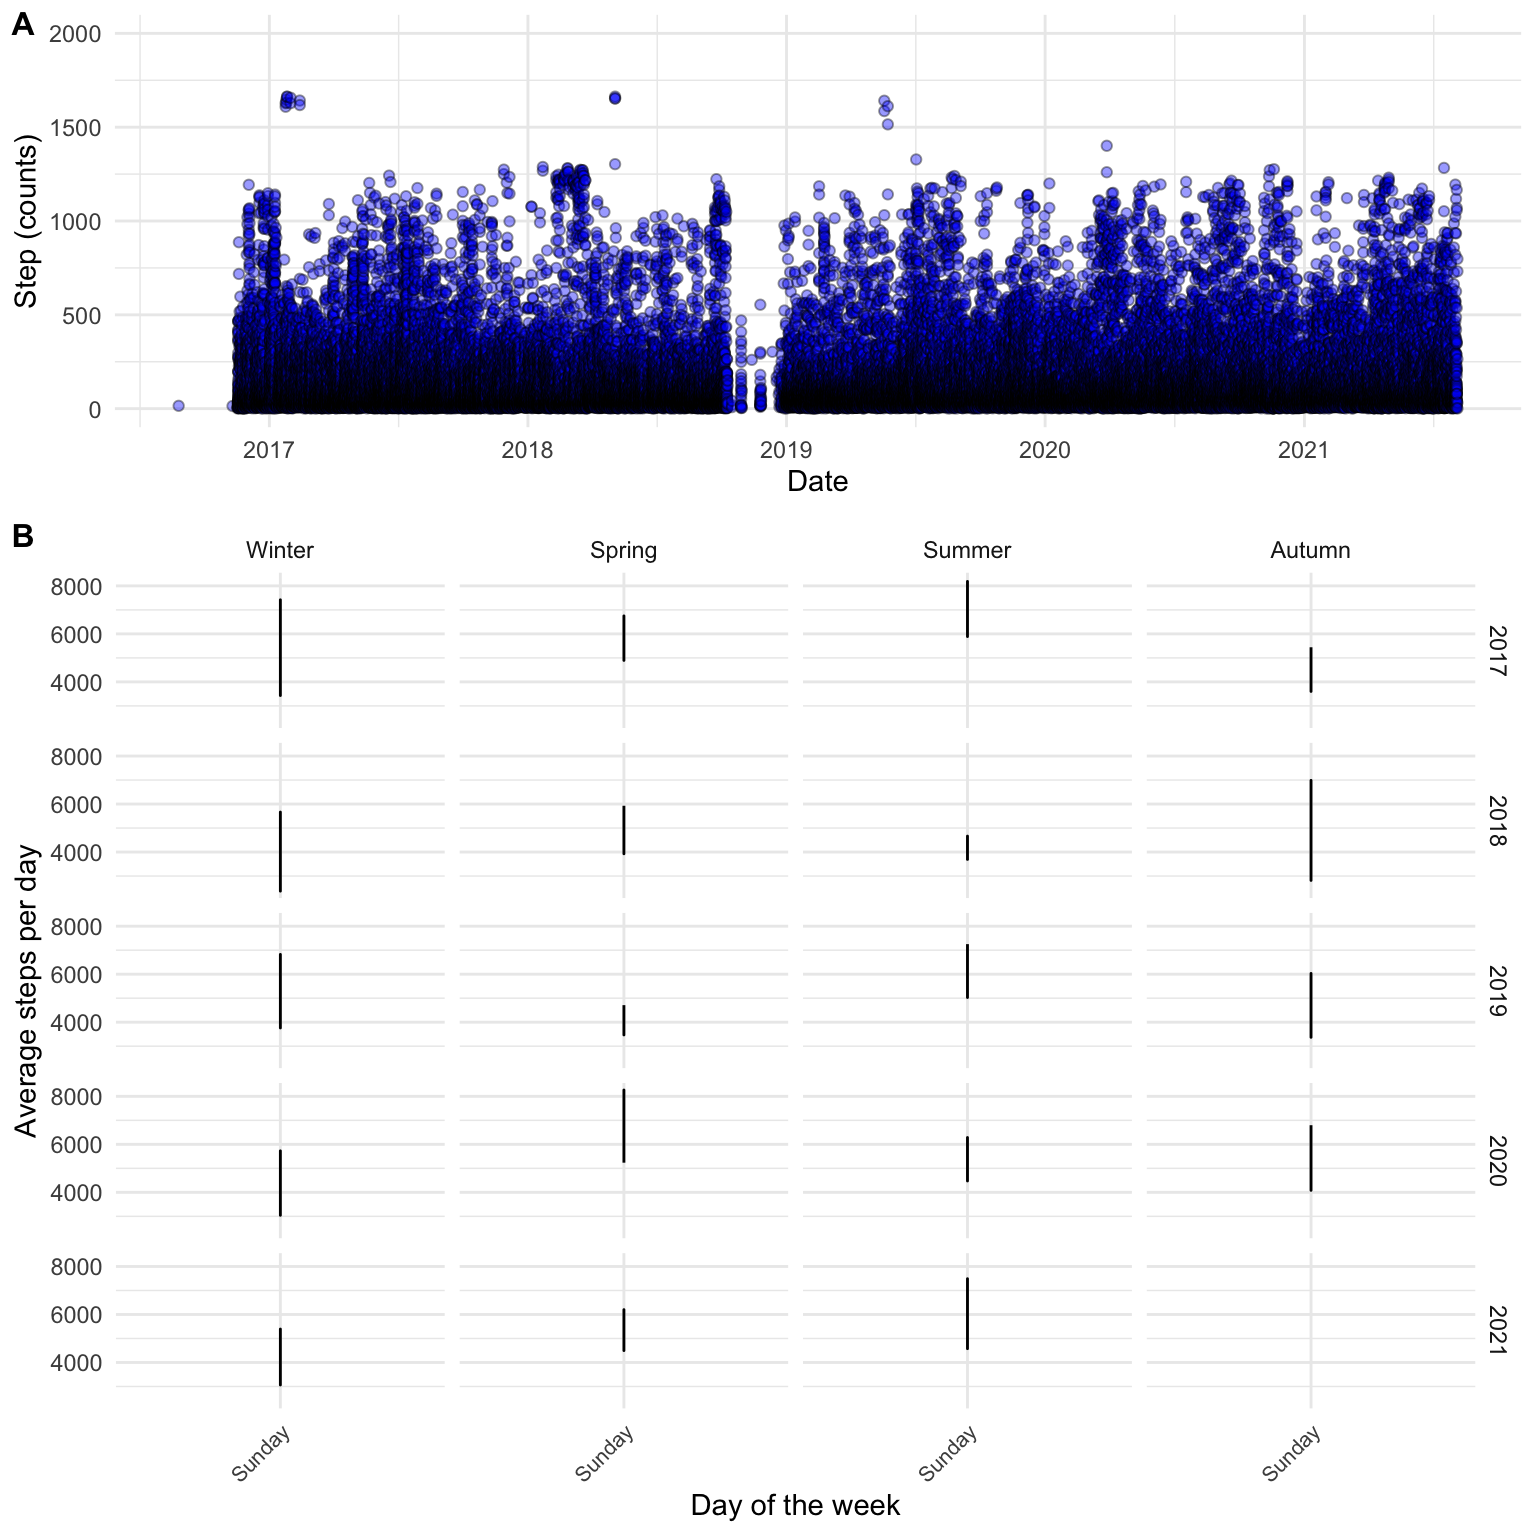
\includegraphics{quant-methods-sport-ex-sci_files/figure-latex/iphone-data-1} 

}

\caption{Step count data from my iPhone displayed as all avalable data points (A, after data cleaning) and average step per weekday, per year and season (B).}\label{fig:iphone-data}
\end{figure}

Data are also collected and stored in publicly available databases. Such databases are created for the purpose to store specific types of data, such as soccer\footnote{\href{https://understat.com/}{understat.com} stores match specific data from major leagues. Data are available through software packages such as \href{https://jaseziv.github.io/worldfootballR/index.html}{\texttt{worldfootballR}}} or biathlon results\footnote{\href{https://biathlonresults.com/}{biathlonresults.com/} hosts results from the international biathlon federation. An example of analyzed data can be \href{https://sciathlon.github.io/post/biathlon_data_analysis/}{seen here}.}, or biological information such as gene sequences\footnote{\href{https://www.ensembl.org/}{Ensembl} and the \href{https://www.ncbi.nlm.nih.gov/}{National center for biotechnology information} are commonly used databases in the biomedical sciences.}. Even data from scientific studies are now days often publicly available\footnote{We published our raw data together with a recent paper (Mølmen et al 2021 \href{https://translational-medicine.biomedcentral.com/articles/10.1186/s12967-021-02969-1}{doi: 10.1186/s12967-021-02969-1.}) together with code to analyze it in a \href{https://github.com/dhammarstrom/rnaseq-copd}{public repository}.} meaning that we can perform scientific studies on unique data sets without collecting the data ourselves.

The above examples shows that there are abundance of data around and available to us. The problem is that it is hard understand all this data. This is where data science and data literacy comes in. In the world of sport and exercise, regardless if you are interested in doing scientific investigations, coach a soccer-team or individual athletes or help patients recover from surgery using exercise therapy, you are faced with the problem of handling and make sense of data. Some of the key skills and deeper understanding about data science are very much transferable between such areas of practice.

\begin{quote}
\textbf{Think about the literature!}
Spiegelhalter (The Art of Statistics, in the introduction chapter) talks about how statistics has evolved towards the broader field of data science. In data science, statistical theory and methods are just parts of the problem solving cycle. Try to think about how you would use the PPDAC cycle as a exercise coach and a scientist. What are the similarities and differences?
\end{quote}

One broader aim of this course is for you to develop skills to better understand data.

\hypertarget{replication-and-reproducibility}{%
\subsection{Replication and Reproducibility}\label{replication-and-reproducibility}}

In scientific research, replication is a way to confirm scientific claims. When a result can be confirmed by an independent group of researchers, the claim is likely ``more true''. Many results will however never be possible to replicate due to the size of trials, costs and urgency of the research question. A recent example could perhaps be the many vaccine trials performed to develop a vaccines against COVID-19\footnote{\url{https://www.evaluate.com/vantage/articles/news/snippets/its-official-covid-19-vaccine-trials-rank-among-largest}}. Other examples concern studies with unique study populations, such as large scale epidemiological studies \citep{RN1492}, but the same could be said to be true for unique investigations in sport and exercise science.

When studies are not likely to be \emph{replicated}, \emph{reproducibility} of the analyses and results has been suggested to be a minimum standard for scientific studies. Reproducibility means that given the same datas, similar results or conclusions can be drawn by independent researchers \citep{RN1492}.

Peng et al. \citep{RN1492} suggests that a \emph{fully reproducible} study has

\begin{itemize}
\tightlist
\item
  Available data.
\item
  Computer code (software) that produces the results of the study.
\item
  Documentation that describes the software and data used in the study, and
\item
  ways to share the data and code.
\end{itemize}

The above principally relates to the trust we can place in scientific results. However, the minimum standard of reproducibility has advantages also for the individual researcher (or master student)! When working with reproducible methods we will develop ways of documenting and automating our analyses. This will make it easier to collaborate with others. And, as it turns out, your most frequent collaborator is you, in the future!

A reproducible data analysis means that you will make it explicit and transparent. In a traditional data analysis, most activities are in the ``black box''. In order to avoid bias \citep{RN1953}, the ``black box'' needs to be opened and you need to actively make transparent decisions all along the analytic pipeline \citep{RN1955}. This pipeline preferably involves the whole problem solving cycle described by Spiegelhalter \citep{RN2902}. However the tools that we will learn about in this course focuses primarily on the steps from the experimental design to presentation of statistical results \citep{RN1955}. These steps includes data collection (and storage), data cleaning, exploratory data analysis, statistical modelling and statistical inference (and communication) \citep{RN1955}.

\hypertarget{tools-in-data-science}{%
\subsection{Tools in data science}\label{tools-in-data-science}}

Ways to interpret and make sense of data involves different methods. These methods are now days often implemented in computer software. This means that when you as a practitioner (scientist, coach, analyst \ldots) want to understand data, you have to master some kind of computer software. The most common software used to understand data is probably Microsoft's Excel. You can do amazing stuff with Excel! In the world of sport and exercise Excel has been used in such diverse activities such as scientific investigations, planning and recording training for Olympic medalists\footnote{The amount of time used by different coaches to create their own specific coaching software really makes many of them amateur software engineers. See for example this training journal from \href{http://obasen.orientering.se/traningsdagbok/installationshandledning.htm}{swedish orienteering}.} and scheduling appointments.

For scientific research, most people use additional software to do statistical analyses. If you have spent time in higher education you have probably heard about SPSS, Stata or Jamovi. These are all specialized software used for statistical analyses.

The above mentioned tools can all be used as part of a fully reproducible workflow. However, there are software solutions that actually suits this requirement better than others. Going back to the description of reproducible science as made by Peng et al. \citep{RN1492}, we want software where analyses can be

\begin{itemize}
\tightlist
\item
  Human- and computer-readable, meaning that we want to be able to write scripts, or computer programs that execute the analyses.
\item
  Documented, meaning that along the code we want to be able to describe what the code does.
\item
  Available and able to share with other, meaning that we analyses can be run on open and free software to maximize ability to share them.
\end{itemize}

This means that the software that we would prefer should be run using scripts (as opposed to point and click) and be free of charge (and open source, as opposed to expensive and proprietary). These criteria can be fulfilled when we use software that is written around the R language (although alternatives exists\footnote{In addition to R, Python offers a free open source environment for reproducible analyses. The choice between the two are \href{https://www.datacamp.com/community/tutorials/r-or-python-for-data-analysis}{matter of taste}.}).

R is a computer language that is especially well suited for reproducible data analysis. As users are able to contribute software extensions, also called packages, many specialized software implementation exists for different tasks, such as creating figures or analyses of specific data. Around R, people have been developing auxiliary software to enable reproducible data analysis. The negative part of all these opportunities is that using R requires some effort. The learning curve is steep!

Even though you might not use R ever again after this course, making and effort trying to learn it will let you know something about programming, capabilities of modern data science, statistical analysis and software/computers in general. These areas are all part of our modern society and are very much transferrable regardless of what computer language we are talking about.

In the next chapter of these course notes we will go through installing and starting up R.

\hypertarget{storing-data-in-spreadsheets}{%
\subsection{Storing data in spreadsheets}\label{storing-data-in-spreadsheets}}

Above, I mentioned spreadsheets like Excel. These are indeed great, but not great for reproducible science or data analysis. This is because they are not easily documented and scripted. The data is actually part of the analysis. Another danger with spreadsheets (like MS Excel) is that it re-formats your data. This is such a big problem for scientists that we have apparently started \href{https://www.theverge.com/2020/8/6/21355674/human-genes-rename-microsoft-excel-misreading-dates}{renaming genes this}. Errors are frequent in spreadsheets, not only because renaming \citep{RN2927}, but also because of bad formatting of formulas \citep{RN2928}. These are both reasons for using spreadsheets only what they are best used for: data input and storage.

\begin{quote}
\textbf{Think about the literature}
Broman and Woo\citep{RN2391} gives several pointers on how to use spreadsheets for data input and storage. Think your experince with Excel, what is the most common mistake you made when handling data in spreadsheets?
\end{quote}

\hypertarget{references-and-footnotes}{%
\subsection{References and footnotes}\label{references-and-footnotes}}

\hypertarget{recording-and-storing-data-in-spreadsheets}{%
\section{Recording and storing data in spreadsheets}\label{recording-and-storing-data-in-spreadsheets}}

\hypertarget{creating-your-first-graph}{%
\section{Creating your first graph}\label{creating-your-first-graph}}

R is an excellent environtment for scientific graphs. There are three main systems for graphical output from R. The first is included in base R.

\hypertarget{creating-your-first-table}{%
\section{Creating your first table}\label{creating-your-first-table}}

\hypertarget{writing-your-first-reproducible-report}{%
\section{Writing your first reproducible report}\label{writing-your-first-reproducible-report}}

  \bibliography{resources/bib.bib}

\end{document}
